\documentclass[11pt]{article}
\usepackage{graphicx}
\usepackage{float}
\usepackage{listings}
\usepackage{hyperref}
\usepackage{caption}
\usepackage{amsmath}
\usepackage{listings}
\usepackage{xcolor}
\usepackage[top = 0.7in,bottom = 1in, left = 0.8in, right = 0.8in]{geometry} 

%New colors defined below
\definecolor{codegreen}{rgb}{0,0.6,0}
\definecolor{codegray}{rgb}{0.5,0.5,0.5}
\definecolor{codepurple}{rgb}{0.58,0,0.82}
\definecolor{backcolour}{rgb}{0.95,0.95,0.92}

%Code listing style named "mystyle"
\lstdefinestyle{mystyle}{
  backgroundcolor=\color{backcolour},   commentstyle=\color{codegreen},
  keywordstyle=\color{magenta},
  numberstyle=\tiny\color{codegray},
  stringstyle=\color{codepurple},
  basicstyle=\ttfamily\footnotesize,
  breakatwhitespace=false,         
  breaklines=true,                 
  captionpos=b,                    
  keepspaces=true,                 
  numbers=left,                    
  numbersep=5pt,                  
  showspaces=false,                
  showstringspaces=false,
  showtabs=false,                  
  tabsize=2
} 
\lstset{style=mystyle}

\title{\textbf{CS747 : Programming Assignment 3}}
\author{\textbf{Adityaya Dhande}   \hspace{8mm} \textbf{210070005}}
\begin{document}
\maketitle

\section*{Approach}
My solution relies on the availability of the \texttt{get\_next\_state} function. 
Here is the algorithm that I implemented in \texttt{agent.py}, 
\begin{enumerate}
    \item For each ball I calculate the angle by the line joining the ball and hole, for all holes
    \item After this I pick a hole which minimises a cost defined as a linear combination of (i)the
    difference in the angle made by the ball-hole line and ball-cue line, and the (ii)distance between ball and hole.
    \item For this I then evaluate the angle at which the cue has to be shot using geometric calculations.
    \item I then take 9 values of force in [0.2, 0.3 $\dots$ 1] and simulate using \texttt{get\_next\_state} function.
    For each \texttt{next\_state} I take the minimum distance of the targeted ball from all holes. I store the minimum of these minimum distances and the corresponding force  
    in separate lists, \texttt{min\_dists} and \texttt{forces} respectively. 
    \item I then select the angle and force corresponding of the ball which corresponds to the 
    minimum of the \texttt{min\_dists} list.

Though in some calls of agent.py I am using the \texttt{get\_next\_state} function more than 
20 times, I'm using it less than 10 times on other ocassions.
I had to tune the linear combination in step 2 for good performance.
\end{enumerate}

\section*{Code explanation}

\begin{lstlisting}[language=Python]      
def cue_dist(self, ballx, bally, cuex, cuey):
    dist = numpy.square(ballx - cuex) + numpy.square(bally - cuey)
    dist = numpy.sqrt(dist)
    return dist

def hole_dists(self, ballx, bally):
    hole_x, hole_y = self.holes[:,0], self.holes[:,1]
    d = numpy.sqrt((hole_x - ballx)**2 + (hole_y - bally)**2)
    return d

def hole_angles(self, ballx, bally):
    hole_x, hole_y = self.holes[:,0], -self.holes[:,1]
    theta_BH = -numpy.arctan2(hole_y + bally, hole_x - ballx) + PI/2
    theta_BH = wrap_angle(theta_BH)
    return theta_BH
\end{lstlisting}
\begin{lstlisting}[language=Python]
def get_delta(self, ballx, bally, hole, d, cue_angle):
    hole_angles = self.hole_angles(ballx, bally)
    hole_angle = hole_angles[hole]
    theta_m = PI/2 - math.asin(self.ball_radius * 2/d)
    angle_error = numpy.clip(hole_angle - cue_angle, -theta_m, theta_m)
    l = numpy.sqrt(d**2 + 4*(self.ball_radius**2) - 4 * d * self.ball_radius * numpy.cos(angle_error))
    shot_angle = numpy.arcsin(2 * self.ball_radius * numpy.sin(angle_error) / l)
    return shot_angle

def simulate(self, ball, delta, current_state):
    forces = numpy.linspace(0.2, 1, 9)
    no_balls = len(current_state.keys())
    curr_min_dist = 2000
    optimal_force = 0.5
    for force in forces :
        next_state = self.ns.get_next_state(current_state, [-delta,force], seed=10)
        if len(next_state.keys()) < no_balls :
            return force, 0
        ballx = next_state[ball][0]
        bally = next_state[ball][1]
        hole_dists = self.hole_dists(ballx, bally)
        min_dist = numpy.min(hole_dists)
        if min_dist < curr_min_dist :
            optimal_force = force
            curr_min_dist = min_dist
    return optimal_force, min_dist
        

def action(self, ball_pos):
    balls = list(ball_pos.keys())
    balls.remove('white')
    if 0 in balls :
        balls.remove(0)
    balls.sort()
    cue_x, cue_y = ball_pos['white']
    X = [ball_pos[i][0] for i in balls]
    Y = [ball_pos[i][1] for i in balls]
    dist = self.cue_dist(X, Y, cue_x, cue_y)
    theta_CB = -numpy.arctan2(cue_y - Y, X - cue_x) + PI/2 
    theta_CB = wrap_angle(theta_CB)
    shooting_angles = []
    forces = []
    min_dists = []
    for i, ball in enumerate(balls) :
        alpha = 0.8
        cost = alpha*self.hole_dists(X[i], Y[i])/600 + (1-alpha)*numpy.absolute(self.hole_angles(X[i], Y[i])-theta_CB[i])
        hole = numpy.argmin(cost)
        delta = self.get_delta(X[i], Y[i], hole, dist[i], theta_CB[i])
        delta = theta_CB[i] - delta
        force, closest_dist = self.simulate(ball, delta/PI, ball_pos)
        shooting_angles.append(delta)
        forces.append(force)
        min_dists.append(closest_dist)
    action = numpy.argmin(numpy.array(min_dists))
    return -shooting_angles[action]/PI, forces[action]
\end{lstlisting}
\noindent
\newpage

\begin{enumerate}
    \item \texttt{cue\_dist} : Returns the distance between 
    \item \texttt{hole\_dists} : Returns the distances between 
    the ball and all the holes in an array. 
    \item \texttt{hole\_angles} : Returns an array containing the angles made by the lines joining the ball 
    with all the holes. 
    \item \texttt{get\_delta} : Returns the $\delta$ angle, as described in \hyperref[sec:Angle_calculation]{angle calculation}
    \item \texttt{simulate} : Returns the best force and the minimum final distance from the closest hole, as described in step 4, for a given ball
    \item \texttt{action} : Evaluates and returns the best action by calling functions to implement 
    the entire algorithm.
\end{enumerate}

\section*{Angle calculation}
\label{sec:Angle_calculation}

\begin{figure}[H]
    \begin{center} 
        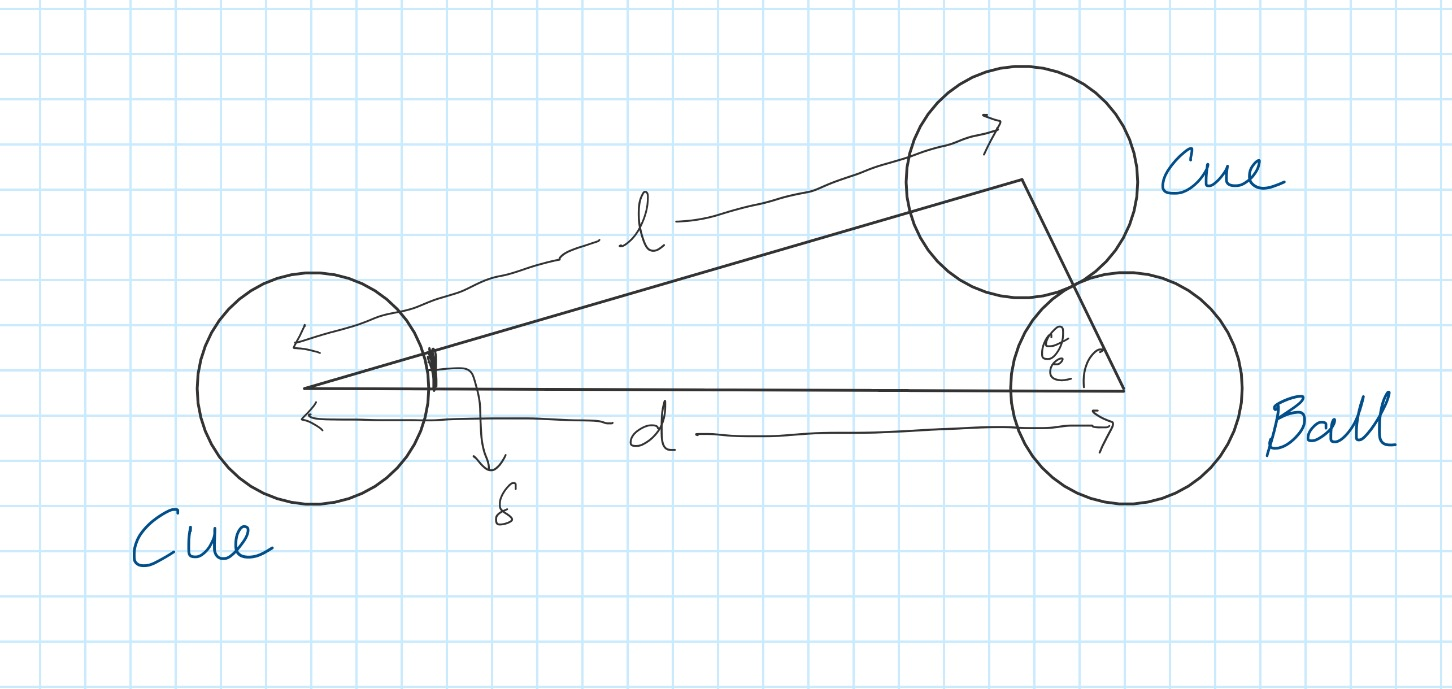
\includegraphics[width=1\textwidth]{screenshot.jpeg}
        \caption*{}
    \end{center}
 \end{figure}
The unknowns in the figure are $l$ and $\delta$. We know $\theta_e$ and $d$ and $r$. 
We can first find $l$ using cosine rule as,
$$ l^2 = d^2 + (2r)^2 - 2 \times(2r) \times(d) \times\cos(\theta_e)$$
We can then use sine rule to find $\delta$ as, 
        $$\sin(\delta) = \frac{(2r)\times \sin(\theta_e)}{l}$$
\end{document}
 